\section{Five branch vertices: reduction and geometry}\label{sec:five-geometry}
Let $B$ be the five original branch vertices and let $S$ be their minimal
connecting subtree. Its leaves belong to $B$, and every vertex of
degree at least three in $S$ belongs to $B$. Suppressing the degree-two
vertices outside $B$ reveals the skeleton. The resulting tree
on five vertices is $P_5$, $K_{1,4}$ or $T_5$: maximum degree four gives
the star, maximum degree three gives degree sequence $(3,2,1,1,1)$,
and maximum degree two gives the path. Each skeleton edge retains its
original positive path length, and every off-core component is a side arm.

At each skeleton vertex $v$, pair equal-length side arms maximally.
Let $c_v$ be its skeleton degree and $t_v$ the number of remaining
distinct arm lengths.
\begin{lemma}\label{lem:five-reduction}
If $c_v+t_v\le2$ at any skeleton vertex, then $U$ has an orientation
satisfying \eqref{eq:kernelbound} for every finite model.
\end{lemma}
\begin{proof}
Orient each equal pair as in \eqref{q3:eq:equalpair}, then bound their
product at $v$ by one in the integrand. The comparison tree retains
$v$, all core paths and the unpaired arms, and has at most four branch
vertices; Theorem~\ref{thm:four-kernel} gives it a fixed orientation.
Restoring the pairs at their original attachment multiplies the
integrand at $v$ by their actual product, which is at most one, so the
original density is also at most one.
\end{proof}
Apply this test at every skeleton vertex. In $P_5$ it covers an empty
internal residual and a terminal with at most one residual arm; an empty
residual at the star or fork center needs the separate argument of
Section~\ref{sec:five-star-fork}.

\begin{figure}[htbp]\centering
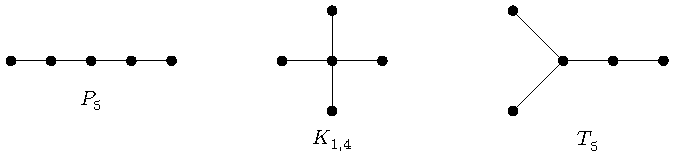
\includegraphics{figures/five-skeletons.pdf}
\caption{The three skeletons on five branch vertices. Every drawn edge denotes an independently chosen positive-length path in the original tree.}\label{fig:five-skeletons}
\end{figure}
